\chapter{Použité metody}

% korelace
% ortogonální
% kontingencni tabulka (vicenasobna)

% zkrtky PCA, MCA, CA,
% znaceni jendotkový vektor rozměru J \mathbf{1}_J
% Singulární rozklad (zkratkou SVD podle anglického názvu Singular Value Decomposition) matice + singulární hodnoty


\section{Redukce dimenzionality} %Extrakce proměnných}

\subsection{Analýza hlavních komponent}

Analýza hlavních komponent (anglicky \emph{Principal component analysis}, dále jako PCA) je statistická metoda využívaná pro pro extrakci proměnných, redukci vícedimenzio-\\nálních dat nebo vizualizaci dat. Lze ji aplikovat pouze na kvantitativní data s numerickými, spojitými hodnotami, neboť metoda využívá lineární algebraické techniky, jako je například kovarianční matice, pro jejíž výpočet se předpokládají spojité hodnoty. 

Jednotlivá pozorování obsažená v datech bývají popsána několika různými příznaky. Tyto příznaky jsou často vzájemně korelované a obsahují šum. Metoda PCA dovede extrahovat pouze důležité informace z proměnných a snížit šum. K~tomu je třeba vypočítat nové ortogonální proměnné, nazývané hlavní komponenty, které se získají jako lineární kombinace původních proměnných \cite{bib:PCA1}. Hlavní komponenty reprezentují směry největšího rozptylu původních dat a jsou řazeny podle své významnosti. Jinými slovy, první hlavní komponenta zachycuje co nejvíce variability v~datech, druhá hlavní komponenta zachycuje co nejvíce variability, která nebyla zachycena první hlavní komponentou, pro zbylé komponenty analogicky. \cite{bib:PCA3}
%, jinými slovy se jedná o přímku,  které nesou největší informaci o datech. Hlavní komponentu si lze představit jako novou osu, která umožňuje vidět data v takovém rozložení, že rozdíly mezi pozorováními jsou lépe patrné.  %https://builtin.com/data-science/step-step-explanation-principal-component-analysis

\subsubsection{Princip}

Předpokládáme množinu dat $\mathbf{X} = (\bm{x}_1, \ldots, \bm{x}_N )$, kde $N$ j počet pozorování a každý vektor $\bm{x}_i$ přísluší jednomu pozorování popsanému $M$ proměnnými. $\mathbf{X}$ je potom matice rozměru $N\times M$ vstupních dat. Dále je definovaný výběrový průměr $\bar{\bm{x}}$ jako
\begin{equation}
    \bar{\bm{x}} = \frac{1}{N} \sum_{i=1}^{N} \bm{x}_i,
\end{equation}
a výběrová kovarianční matice $\mathbf{C}$

\begin{equation}
    \mathbf{\mathbf{C}} = \frac{1}{N} \sum_{i=1}^{N} (\bm{x}_i - \bar{\bm{x}}).
\end{equation}

První hlavní komponentu, která popisuje největší rozptyl dat označíme $y_{1i}$ a vypočteme následovně jako lineární kombinaci původních proměnných
\begin{equation}
    y_{1i} = \bm{a}_1^\top (\bm{x}_i - \bar{\bm{x}}), \quad \mbox{pro } i=1,\ldots,N,
\end{equation}
kde $\bm{a}_1 = (a_{11}, \ldots, a_{M1})^\top $ je vektor vah. 

Optimální vektor $\bm{a}_1$ je takový vektor, který maximalizuje výběrový rozptyl nové proměnné $y_{1i}$ za podmínky $\bm{a}_1^\top\bm{a}_1 = 1$. Pakliže je výběrový rozptyl $y_{1i}$ definován jako 
\begin{equation}
    D(y_{11}, \ldots, y_{1N}) = \bm{a}_1^\top \mathbf{C} \bm{a}_1
\end{equation}
můžeme maximalizační úlohu vyřešit pomocí metody Lagrangeových multiplikátorů. Lagrageova funkce s parametrem $\lambda_1$ má následující tvar
\begin{equation}
    \mathcal{L}(\bm{a}_1, \lambda_1) = \bm{a}_1^\top \mathbf{C} \bm{a}_1 - \lambda_1(\bm{a}_1^\top\bm{a}_1 - 1).
\end{equation}

Derivaci funkce položíme rovnou nule 
\begin{align*}
    \frac{\partial \mathcal{L}}{\partial \bm{a}_1}  = 2 \mathbf{C} \bm{a} - 2\lambda_1 \bm{a}_1 \overset{!}{=}  0 \\
    (\mathbf{C} - \lambda_1 \mathbf{I} ) \bm{a}_1 \overset{!}{=}  0,  \\
\end{align*}
kde $\mathbf{I}$ je jednotková matice.

Řešíme soustavu lineárních rovnic pro neznámý parametr $\bm{a}_1$, která má řešení právě tehdy, když je matice $\mathbf{C} - \lambda_1 \mathbf{I} $ singulární, tedy platí, že její determinant  je roven nule. $\lambda_1$ je pak největší vlastní číslo matice $\mathbf{C}$ a $\bm{a}_1$ vlastní vektor příslušný tomuto vlastnímu číslu. Toto tvrzení se matematicky zapíše následovně
\begin{equation}
    \mathbf{C} \bm{a}_1 = \lambda_1 \bm{a}_1. \\
\end{equation}
Po vynásobení vektorem $\bm{a}_1$ zleva získáme řešení pro maximální rozptyl proměnné $y_{1i}$
\begin{equation}
    D(y_{11}, \ldots, y_{1N}) = \bm{a}_1^\top \mathbf{C} \bm{a}_1 = \lambda_1.
\end{equation}


Druhá hlavní komponenta
\begin{equation}
    y_{2i} = \bm{a}_2^\top (\bm{x}_i - \bar{\bm{x}}), \quad \mbox{pro } i=1,\ldots,N,
\end{equation}
se vypočte obdobným způsobem s přidanou podmínkou ortogonality vzhledem~k první hlavní komponentě -- druhá hlavní komponenta nesmí být korelovaná s předchozí, první hlavní komponentou. Potom popisuje druhý největší možný rozptyl v datech. Znázornění dvou hlavních komponent ve dvoudimenzionálním prostoru je vyobrazeno na obrázku \ref*{obr:met:PCA1}.
Vektor  $\bm{a}_2$ se opět získá jako jednotkový vlastní vektor kovarianční matice $\mathbf{C}$ příslušící druhému největšímu vlastnímu číslu $\lambda_2$.\cite{bib:PCA1, bib:PCA3} %https://builtin.com/data-science/step-step-explanation-principal-component-analysis

\begin{figure}[hbtp!]
    \centering
    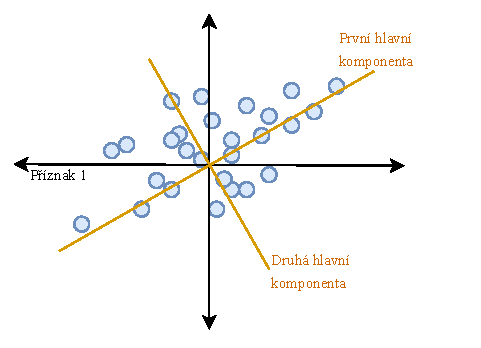
\includegraphics[width=\textwidth]{obrazky/PCA.pdf}
    \caption{Znázornění dvou hlavních komponent na pro dvě proměnné. Zdroj: vlastní.}
    \label{obr:met:PCA1}
\end{figure}


Získání předpisů pro další hlavní komponenty je analogické. Obecně lze zapsat metodu PCA a převod původních proměnných následujícím maticovým zápisem
\begin{equation}
    \mathbf{Y} = \mathbf{XA}, 
\end{equation}
kde $\mathbf{X}$ je matice vstupních dat, $\mathbf{A}$ je matice vlastních vektorů kovarianční matice $\mathbf{C}$. Pro matici $\mathbf{A}$ zároveň platí $\mathbf{C} =  \mathbf{A} \mathbf{\Lambda} \mathbf{A}^\top$, kde $\mathbf{\Lambda}$ je diagonální matice vlastních čísel $\mathbf{C}$.\cite{bib:PCA2}  %wikipedia

\subsection{Korespondenční analýza}

Vícenásobná korespondenční analýza (anglicky \emph{Multiple correspondence analysis}, dále jako MCA) je metoda, která umožňuje popsat vztahy mezi daty, které jsou popsané kategorickými proměnnými, vytvořením kontingenční tabulky. V případě, že se popisuje vzájemná relace pouze dvou proměnných, se použije základní korespondenční analýza\footnote{anglicky \emph{correspondence analysis} (CA)}. MCA je alternativou~k PCA, pokud jsou analyzovanými daty kategorická data. \cite{bib:MCA1}

% \subsubsection{Princip korespondenční analýzy}
\subsubsection{Značení}
%https://statmath.wu.ac.at/courses/CAandRelMeth/caipA.pdf
Nechť $\mathbf{N}$ je matice dat s rozměry $I\times J$, kde I odpovídá počtu pozorování a J je počet kategorií. %asi pocet kategorii, najit !!!
Matice $\mathbf{N}$ je převedena na korespondenční matici $\mathbf{P}$ vydělením matice $\mathbf{N}$ jejím celkovým součtem $n = \sum_{i=1}^{I} \sum_{j=1}^{J} n_{ij}=\mathbf{1}^\top_I \mathbf{N}\mathbf{1}_J$. To zaručuje, že součet prvků matice $\mathbf{P}$ je roven jedné. Tyto kroky lze shrnout následujícím matematickým zápisem
\begin{equation}
    \mathbf{P} = \frac{1}{n}\mathbf{N}, \qquad \mathbf{P} = \{p_{ij}\},  \qquad  \sum_{i=1}^{I} \sum_{j=1}^{J} p_{ij} = 1.
\end{equation}
Součet $i$tého řádku, resp. součet $j$tého sloupce je značen následovně
\begin{align*}
    r_i = \sum_{j=1}^{J} \qquad \mbox{ pro } i=1,\ldots,I, \\
    c_j = \sum_{i=1}^{I} \qquad \mbox{ pro } j=1,\ldots,J.
\end{align*}
Vektor $\bm{r} = \mathbf{P} \mathbf{1}_J $ obsahuje všechny řádkové součty matice $\mathbf{P}$, analogicky vektor $\bm{c} = \mathbf{P}^\top \mathbf{1}_I $ obsahuje všechny sloupcové součty téže matice.

Pro další výpočty zavedeme značení pro diagonální matice, které mají na diagonále  řádkový, resp. sloupcový součet
\begin{equation}
    \mathbf{D}_r = \mbox{diag}(\bm{r}), \quad \mbox{ resp. } \quad \mathbf{D}_c = \mbox{diag}(\bm{c}).
\end{equation}

% Pro připomenutí je vhodné dodat, že součet matice P je jedna

\subsubsection[Výpočetní algoritmus základní korespondeční analýzy]{Výpočetní algoritmus základní korespondeční analýzy \cite{bib:CA1,bib:MCA2}}
Označme $\mathbf{S}  = \{s_{ij}\}$ následující matici
\begin{equation}
    \mathbf{S} := \mathbf{D}_r^{-\frac{1}{2}} (\mathbf{P} - \bm{rc}^\top) \mathbf{D}_c^{-\frac{1}{2}}.
\end{equation}
Po té proveďme singulární rozklad této matice
\begin{equation}
    \mathbf{S} = \mathbf{U}\mathbf{\Delta}\mathbf{V}^\top,
\end{equation}
kde $\mathbf{\Lambda} = \mathbf{\Delta}^2$ je matice vlastních čísel $\lambda_k$ pro $k=1,\ldots,K$, kde $K=min\{I-1,J-1\}$. Potom rozměry matice $\mathbf{U}$, resp. $\mathbf{V}$ jsou $I\times k$, resp.  $J\times k$. Dále platí $\mathbf{U}^\top\mathbf{U}=\mathbf{V}^\top\mathbf{V}=\mathbf{I}$.%https://www.wikiwand.com/en/Correspondence_analysis


% Zatímco u PCA je měřítkem úspěchu míra rozptylu popsaná prvními vybranými hlavními komponentami 
Korespondenční analýza měří míru váženého rozptylu, tzv. inercii pomocí vlastních čísel $\lambda_k$ matice $\mathbf{S}$, $\lambda_k$ se pak nazývají hlavní inercie.
Celková inercie je rovna
\begin{equation}
    I = \sum_{k=1}^{K} \lambda_k = \sum_{i=1}^{I}\sum_{j=1}^{J} s_{ij}^2.
\end{equation}

Hlavní komponenta řádků $\mathbf{F}$ je rovna
\begin{equation}
    \mathbf{F} = \mathbf{D}_r^{-\frac{1}{2}} \mathbf{U}  \mathbf{\Delta}.
\end{equation}
Hlavní komponenta sloupců $\mathbf{G}$ je rovna
\begin{equation}
    \mathbf{G} = \mathbf{D}_c^{-\frac{1}{2}} \mathbf{V}  \mathbf{\Delta}
\end{equation}

\subsubsection*{Výpočetní algoritmus MCA}

Předpokládejme, že původní matice kategorických dat má tvar $N\times Q$, tj. $N$ pozorování a $Q$ proměnných. Matici dat převedeme na indikátorovou matici. Indikátorová matice  $\mathbf{Z} $ je vytvořena tak, že kategorická data jsou rozepsána do pomocných proměnných. Pokud $q$tá proměnná je má $J_q$ typů kategorií, tak příslušná indikátorová matice bude mít $J = \sum_{q=1}^{Q}J_q$ sloupců a $N$. Tzn. počet proměnných byl tímto rozepsáním rozšířen z počtu původních $Q$ proměnných na $J$ proměnných.
% Klasická MCA má dvě podoby.
První způsob MCA aplikuje základní algoritmus korespondenční analýzy na matici  $\mathbf{Z}$, takto se získají souřadnice pro N pozorování a J kategorií.

% https://towardsdatascience.com/famd-how-to-generalize-pca-to-categorical-and-numerical-data-2ddbeb2b9210 
% https://arrow.tudublin.ie/cgi/viewcontent.cgi?article=1227&context=scschcomdis

% \subsection{Particle Swarm Optimization}

% https://www.analyticsvidhya.com/blog/2021/10/an-introduction-to-particle-swarm-optimization-algorithm/

\subsection{Korelační analýza}

\subsubsection{Korelační koeficient}
\subsubsection{Další způsoby měření závislosti}

Pro určení kolik informace o jedné proměnné nese druhá proměnná, je popsáno
pomocí vzájemné informace \cite{bib:MI}. Informací lze rozumět obsah jakéhokoli oznámení nebo údaje, který se přenáší v daném čase a prostoru. Podle Shannona, zakladatele teorie informace, je informace míra množství neurčitosti nebo nejistoty o nějakém náhodném jevu, která se odstraní realizací daného jevu \cite{bib:MI2}. Informací tak může být stanovení výsledku náhodného jevu, tedy se jedná o hodnotu náhodné veličiny \cite{bib:MI}. Pro definování vzájemné informace je třeba definovat ještě vlastní informace a pojem entropie.

Dále jsou sepsány předpoklady pro výpočet množství informace. Pokud má náhodný jev $X$ $n$ realizací, pak je množství informace funkcí $n$. Pakliže je $n=1$, množství informace se rovná nule, neboť se jedná o jev jistý. 
Pokud jevy $X$ A $Y$ probíhají nezávisle, ale ve stejný čas, tj. $p(x,y)$, potom množství informace obou jevů se tovná součtu jejich množství.
Pokud jev $X$ má $n $ realizací a jev $Y$ $m$ realizací, kde $m>n$, potom se očekává, že množství informace jevu $Y$ je větší než množství informace jevu $X$. \cite{bib:MI2}


Entropie náhodného jevu $X$, který má $n$ realizací $X = x_1, x_2, \ldots, x_n$ s pravděpodobnostmi $X = p(x_1), p(x_2), \ldots, p(x_n)$

Theilovo U a Cramerovo V
%https://www.statology.org/interpret-cramers-v/
rozptylový inflační faktor (VIF)

\subsection{Metoda GUHA}
\label{sec:Teorie:Guha}
Uvažujeme potenciálně nekonečnou množinu objektů. Metoda předpokládá výsledky existenci pozorování této množiny reprezentované v matici dat. Cílem je získat všechny zajímavé vztahy, které jsou pravdové pro celou množinu objektů

Tvrzení pravdivé o celé množině objektů verifikovaným teoretickým tvrzením. Tvrzení na datech z pozorování nazýváme observačním tvrzením. Důležité je, že mezi teoretickými a observačními tvrzeními obvykle platí vztah 1:1. Tento vztah je zprostředkován statistickými testy hypotéz.

GUHA procedura generuje a verifikuje napozorovaná data s množinou možných relevantních tvrzení, výstupem jsou potom všechna prostá observační tvrzení. \textit{Relevantní tvrzení je prosté, je-li pravdivé v daných datech a zároveň neplyne zjevným způsobem z jiného, kratšího a ve výstupu již uvedeného tvrzení.} % přepsat větu....!!!

Metoda pracuje s nádledujícími pojmy

\begin{itemize}
    \item Matice dat a atributy - Řádky matice jsou jednotlová pozorování. Atributem se rozumí sledovaná vlastnost, jedná se o sloupec matice.
    \item Základní booleovský atribut - Jedná se o výraz A(a), kde A je atribut a $a$ je vlastní pdomnožina A. $a$ může obsahovat více prvků než jeden.
    \item Booleovský atribut -  Každý zákl. b. atribut je booleovský atribut. Boolovské atributy jsou negace, konjunkce a disjunkce základních boolovských atributů.
    \item Literál - Zákaldní boolovský atribut nebo jeho negace
    \item Dílčí cedent - jedná se o konjunkci nebo disjunkci literálů.
    \item Cedent - Jedná se o konjunkci dílčích cedentů. Příkladem cedentu je booleovský atribut.
\end{itemize}

\subsubsection*{Procedury}

4ft-Miner pracující s GUHA asociačními pravidly a s podmíněnými GUHA asociačními pravidly $\phi \approx  \psi / \chi $

Asociační pravidlo -  Asociačním pravidlem se tedy obvykle rozumí výraz A $\leftarrow$ S kde A i S jsou konjunkce dvojic atribut-hodnota. %!!! přepsat větu

Konfidence asociačního pravidla A $\leftarrow$  S je podíl (počet řádků splňujících A i S)/(počet řádků splňujících S)  %!!! přepsat větu


% Procedura 4ft-Miner pracuje s GUHA asociačními pravidly φ≈ψ kde φ a ψ jsou booleovské atributy. Pravidlo φ≈ψ je pravdivé v matici dat M, pokud φ a ψ jsou v matici dat M ve vztahu daném 4ft-kvantifikátorem ≈. Každý 4ft-kvantifikátor definuje podmínku týkající se kontingenční tabulky φ a ψ. GUHA asociační pravidla jsou obecnější než asociační pravidla produkovaná známým algoritmem apriori. Je možno pracovat i s podmíněnými GUHA asociační pravidly φ≈ψ/χ kde χ je booleovský atribut.

% \subsection{Genetický algoritmus}

% Genetický algoritmus byl inspirovaný evoluční teorií a přirozeným výběrem. Je založený na teorii, že jedinci, kteří jsou lepší než ostatní mají větší šanci na to, předat svou genetickou informaci dál. Jejich geny tk budou základem nové generace. Podobně jako ve zmíněné teorii, algoritmus používá následující informace: genetickou reprezentaci pomocí bitového  řetězce, funkci pro vyhodnocení tzv. fitness funkci, kombinování genů a mutaci. 

% Nejprve se vytvoří náhodná populace. Od této inicializační populace se postupně se iteruje dokud již další změny nevedou k lepšímu řešení, nebo dokud neskončí počet iterací. Jedna iterace je analogií k jedné evoluční generaci.

% Bitový řetězec populace se vyhodnotí pomocí cílové funkce (objective function). Hodnota cílové funkce pak určuje hodnotu fitness daného řešení. Fitness je možné uvažovat jako minimalizační nebo maximalizační kritérium.

% Dále se vyberou dva rodiče podle své fitness hodnoty, kteří se mezi sebou zkříží a jejich potomek vstoupí do další iterace. Jeden ze způsobů výběru je vybrat k náhodných populací a znich vybrat populaci s nejvyšším fitness. Křížení rodičů je pravděpodobnostní, takže v některých případech ,ůže vzniknout potomek stejný jako jeho rodič. Obvykle se hyperparametr pro křížení se nastavuje na vyšší hodnoty např. 80 nebo 90 \%. Dalším parametrem je mutace, ta určuje zda přenesený bit zmutuje nebo ne. Jeho hodnota se nastavuje jako $1/L$, kde $L$ je délka řetězce.



